Der Großteil, neben der Feldarbeit, dreht sich bei der Landwirtschaft um den
Viehbetrieb. Hier gibt es bereits einige Automatisierungen, wie zum Beispiel
Melkstraßen, wo Kühe mithilfe von Melkrobotern nacheinander vollautomatisch
gemolken werden. Was zudem sehr leicht zu automatisieren ist, ist die Ernährung
jeglicher Tierarten.\\ Man benötigt lediglich ein System, das Futter von großen
Lagerbehältern zu den Ställen/Gehegen bringt. Das kann je nach Bauernhof
unterschiedlich aussehen. Die einfachste Umsetzung wäre hierbei meiner Hinsicht
nach ein höher gelegenes Schienensystem. Damit gibt es keine Behinderung der
sonstigen Arbeit, und man kann das komplette System mittels eines
Mikrokontrollers, wie zum Beispiel eines Raspberrys, steuern. Die
herkömmlichsten Roboter gleichen jedoch herkömmlichen Futtermischwägen, welche
vollautomatisiert durch die Ställe fahren. (Abb. 5.1)

\begin{figure}[ht]
    \centering
    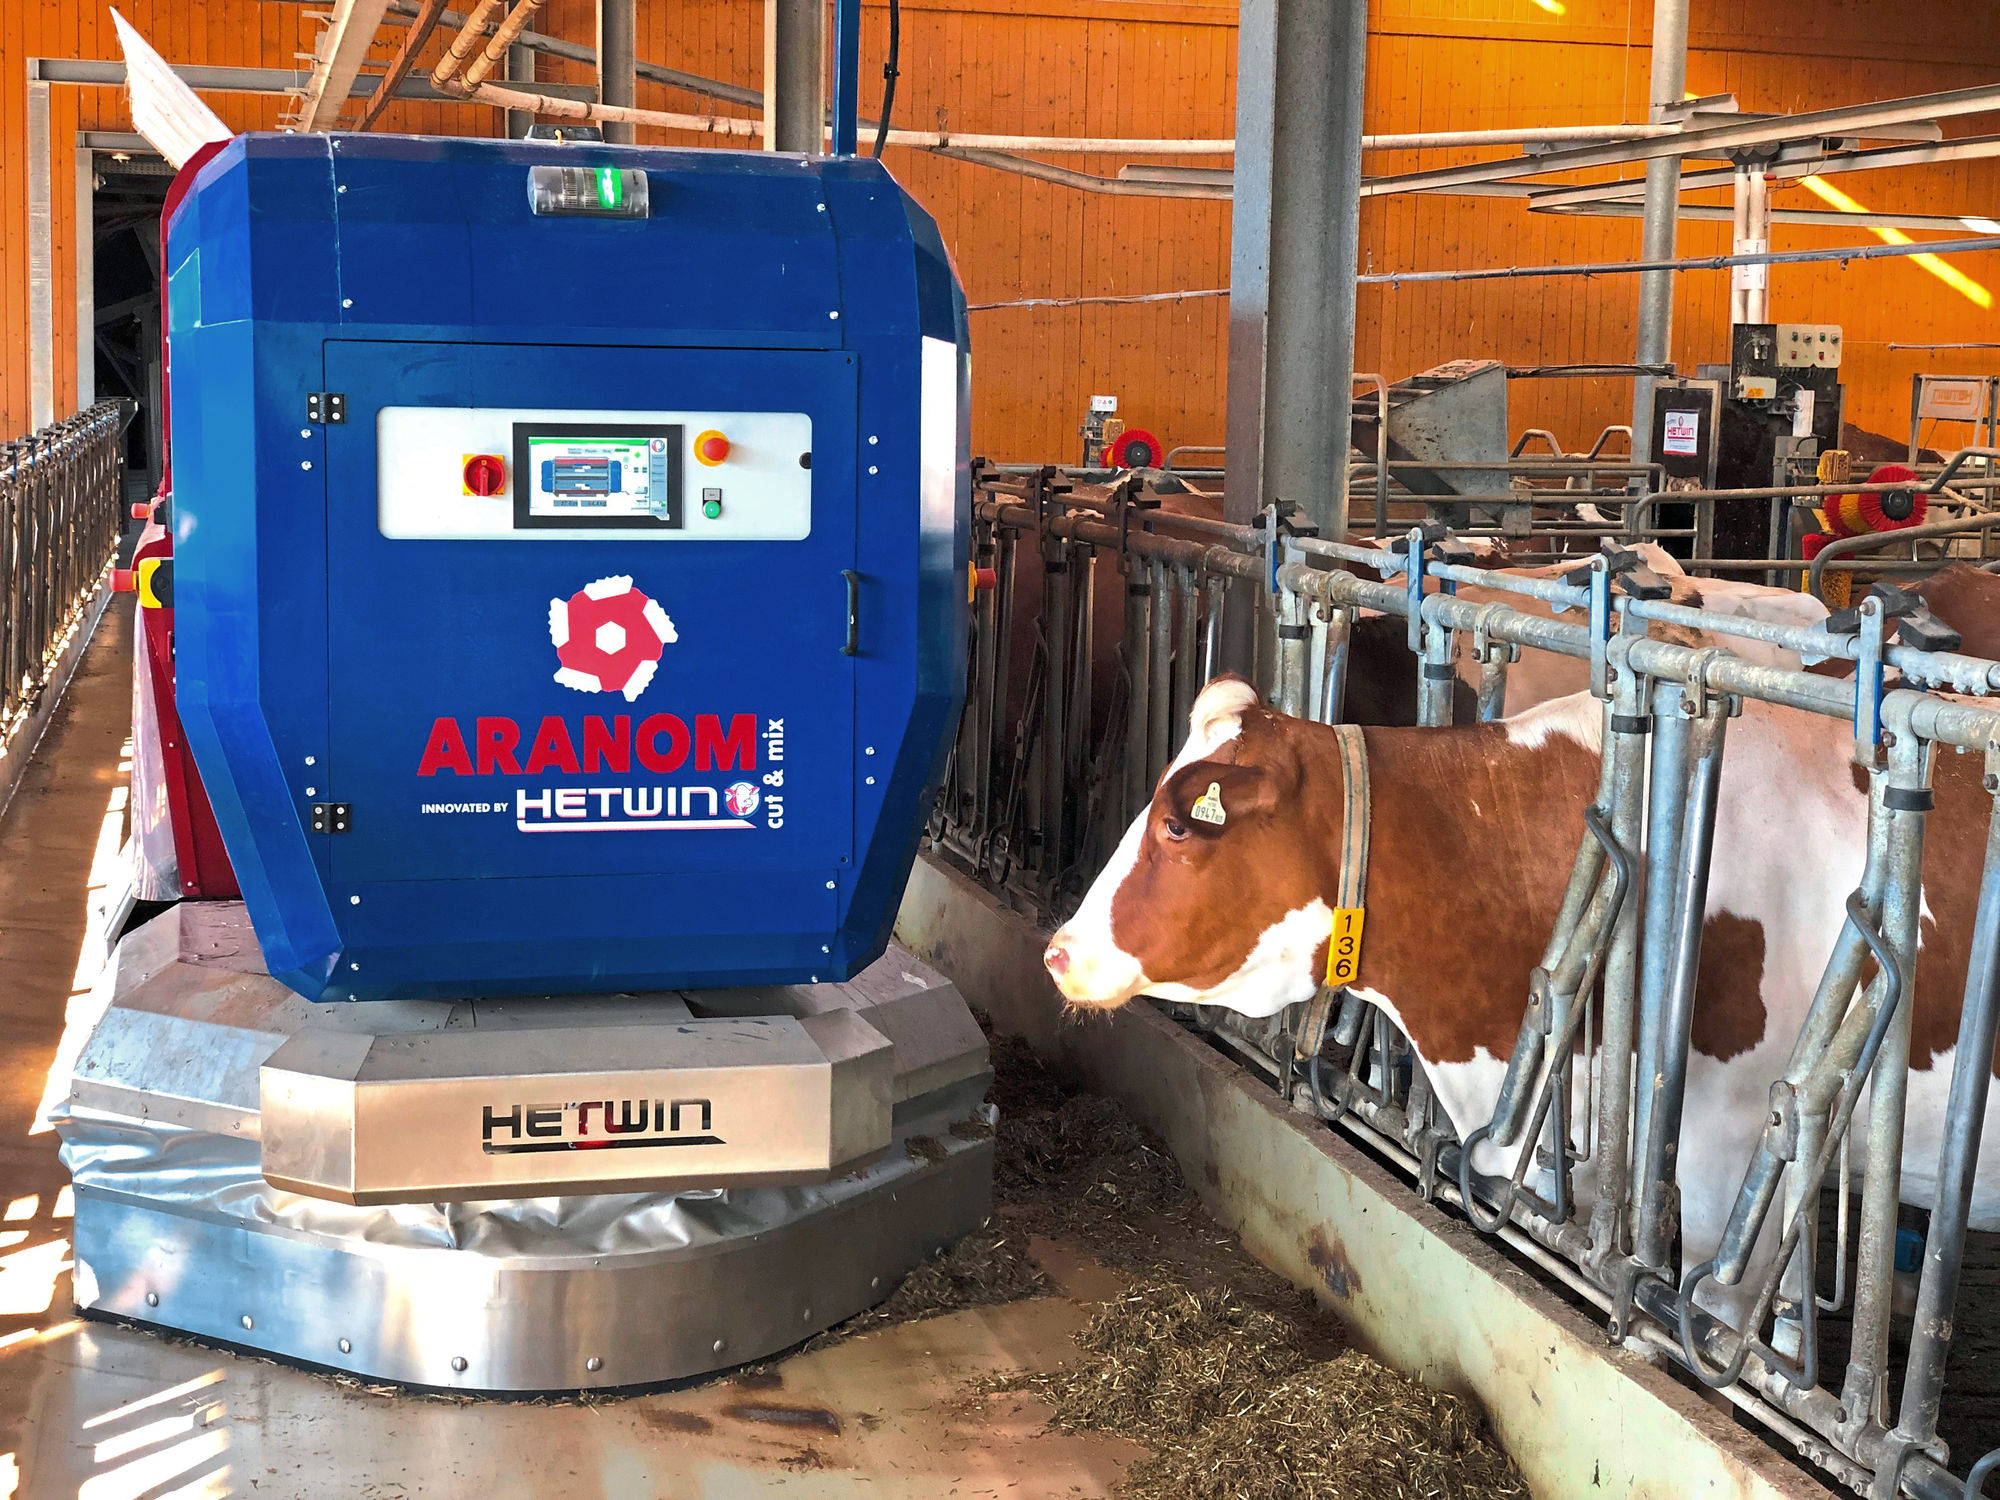
\includegraphics[width=0.7\textwidth]{bilder/futterroboter.jpg}
    \caption[Futterroboter in Kuhstall]{Futterroboter in Kuhstall}
    \label{fig:futterroboter}
\end{figure}